\chapter{The LHCb detector}
\label{chap:dec}
In this section, overview of accelator complex at CERN as well as physics motivation behind \Gls{LHCb} detector and its details will be described.

CERN built one of the most exciting laboratories to study elementary particle interactions. The complex set of particle accelerators and detectors is shown in \autoref{fig:AcceleratorComplex}. The proccess of accelerating protons starts with the source of protons. Protons are obtained from hydrogen gas bottle by applying and an electric field seperates hydrogen into positively and negatively charged constituents. The first proton accelerator in the chain, Linac 2, accelerates the protons to the energy of 50 MeV. Is is a tank composed of several chambers where the resonant cavity is tuned to a specific frequency which creates potential differences in the cavities making accelerate the protons. These are then injected into the Proton Synchrotron Booster (PSB). Here the protons are accelerated to 1.4 GeV. The next line is the Proton Synchrotron (PS) reaching energy of 25 GeV. Before either entering the LHC or North Area (mainly used as testing facility for experiment upgrades) Super Proton Synchrotron (SPS) is the last stop. Here proton acceleration to 450 GeV is achieved.

\begin{figure}
  \centering
  \includegraphics[scale = 1.0]{figs/detector/AccComplex.png}
	\caption{Accelerator complex at CERN. The image is taken from \cite{complex}.}
  \label{fig:AcceleratorComplex}
\end{figure}

The Large Hadron Collider (LHC) is a complex machine which accelerates beams of protons in opposite directions in $\sim$ 27km circular tunnel. It is located
50-157\m below ground on the border of Switzerland and France. Once the desired energy is achieved proton-proton, $pp$, or ion, collisions happen at four distinct points, where different detectors with different physics focus are located. These are \Gls{ATLAS}, \Gls{CMS}, \Gls{ALICE} and \Gls{LHCb}. 
Study of \Bmumumu was performed using data obtained at \Gls{LHCb}. 

\section{LHCb Layout}

\Gls{LHCb} differs from the other general purpose detectors on the LHC ring as its studies properties of heavy particles containing $b$ or $c$ quarks. This can be attributed to the geometrical acceptance and unique vertex resolution as well as excelent \Gls{PID}.

Contrary to the two general purpose detectors where the collisions are occuring in the centre of the detector, \Gls{LHCb}'s collision point is located at one end of the detector, hence its description as a forward single-arm spectrometer. This means that information about products outside of its scope are not known, meaning that there is no overall constraint on collision information, unlike in other flavour experiments. This is compensated by production mechanism of $b\bar{b}$ and $c\bar{c}$ in $pp$ interactions, which occurs via gluon-gluon fusion. In this process, each gluon will carry part of proton's momentum. If the two gluons from two protons carry significantly different momentum, the $b\bar{b}$ system will be boosted with respect to the $pp$ rest frame, either in forward or backward cone closely to the beamline, as can be seen in \autoref{fig:Acceptance}.

\begin{figure}
	\centering
	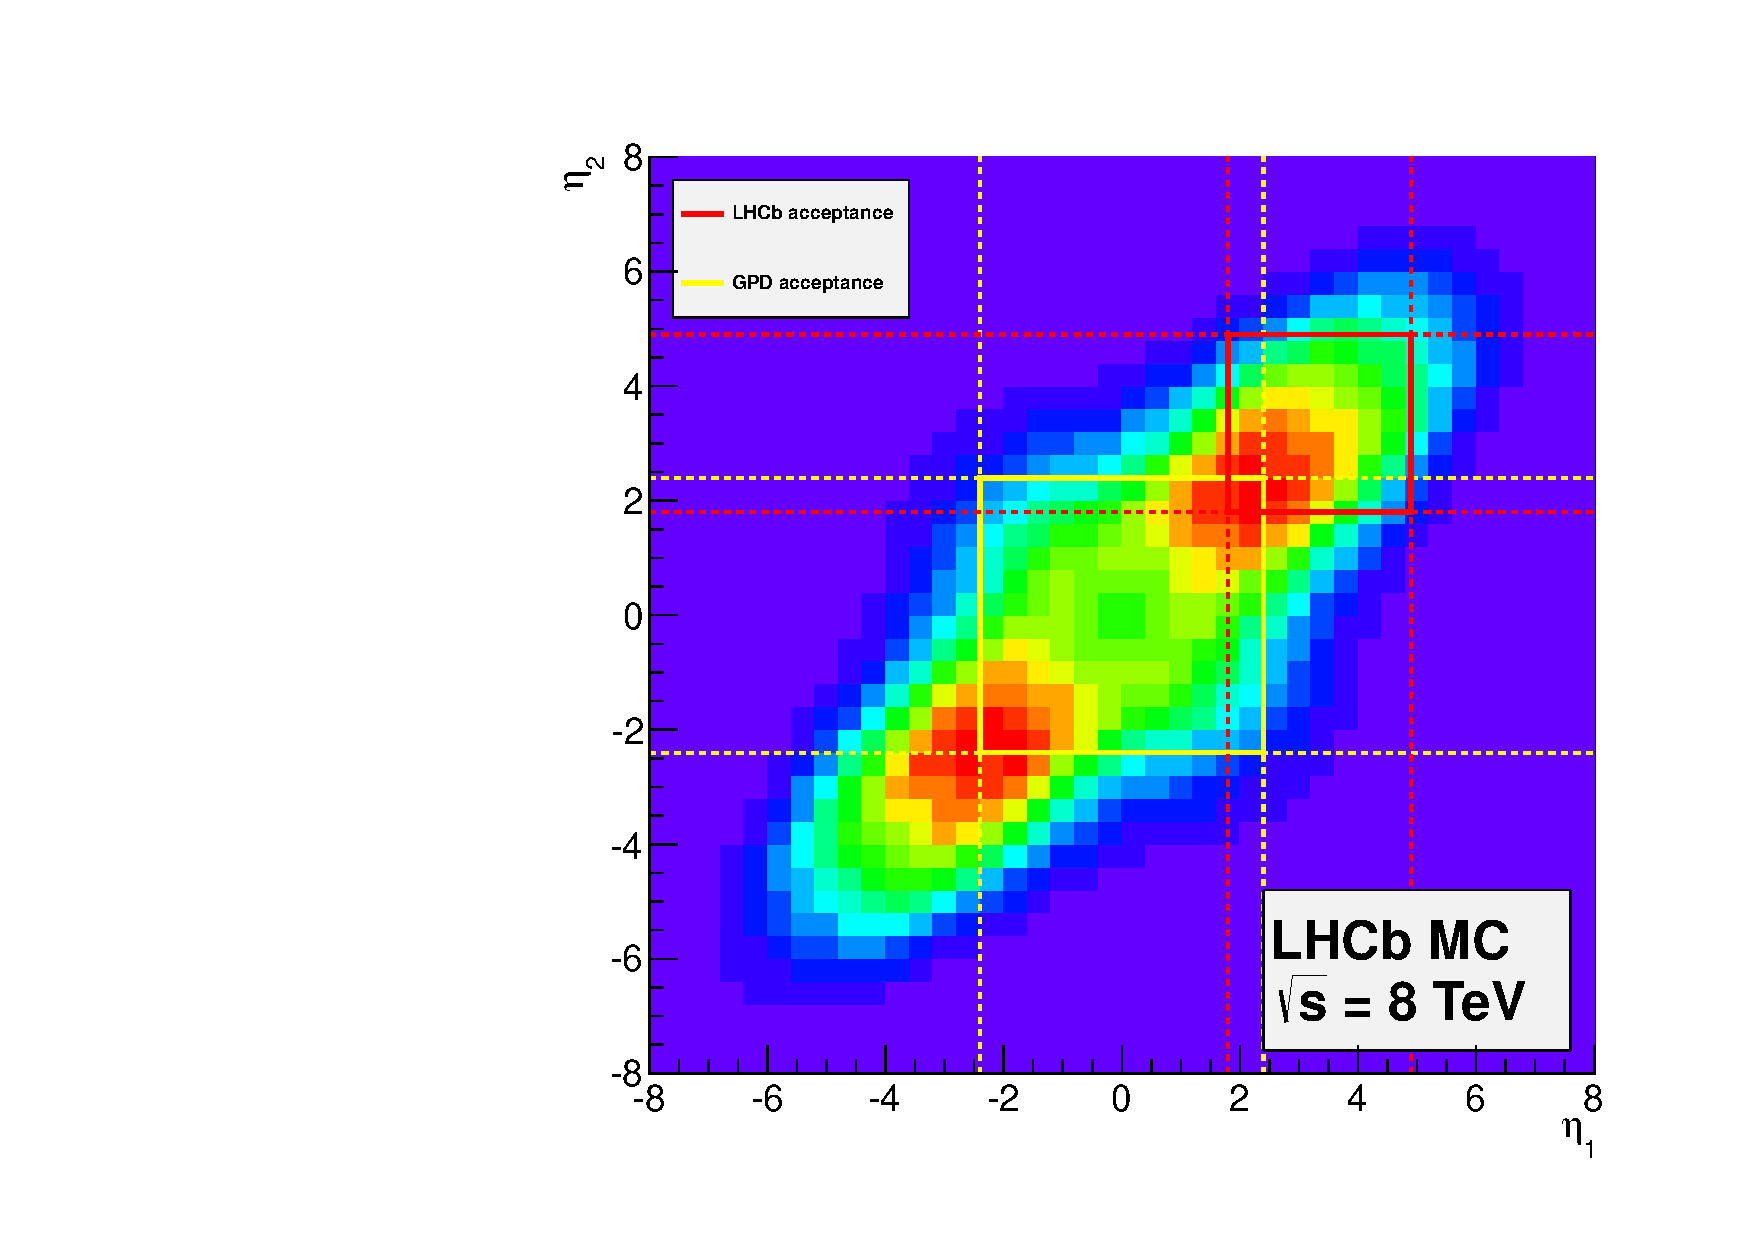
\includegraphics[scale = 0.3]{figs/detector/Acceptance.pdf}
	\caption{Angular production and acceptance of LHCb's $b\bar{b}$ pair (in red) as well as General Purpose Detector (in yellow). LHCb covers region with highest production cross-section at 8 \tev. These plots were produced using PYTHIA8 \cite{pythia8} simulation. This plot was taken from \cite{acceptance}.}
	\label{fig:Acceptance}
\end{figure}

The angular coverage of LHCb is formally defined using pseudorapidity $\eta$, 

\begin{equation}
	\eta = -\ln (\tan\frac{\theta}{2})
\end{equation}	
where $\theta$ is defined in \autoref{fig:LHCbDetector}. \Gls{LHCb} detector, hence, covers the region $2<\eta<5$. The production cross-section of the fundamental process of $pp\rightarrow b\bar{b}X$ was measured in this region yielding, $\sigma (pp\rightarrow b\bar{b}X)$= 75.3$\pm$5.4$\pm$13.0 $\upmu$b at 7 \tev \cite{LHCb-PAPER-2010-002} and 144$\pm$1$\pm$21 $\upmu$b at 13 \tev \cite{LHCb-PAPER-2016-031}, which shows that the production cross-sections scales roughly linearly with the centre-of-mass energy.

\begin{figure}
	\centering
	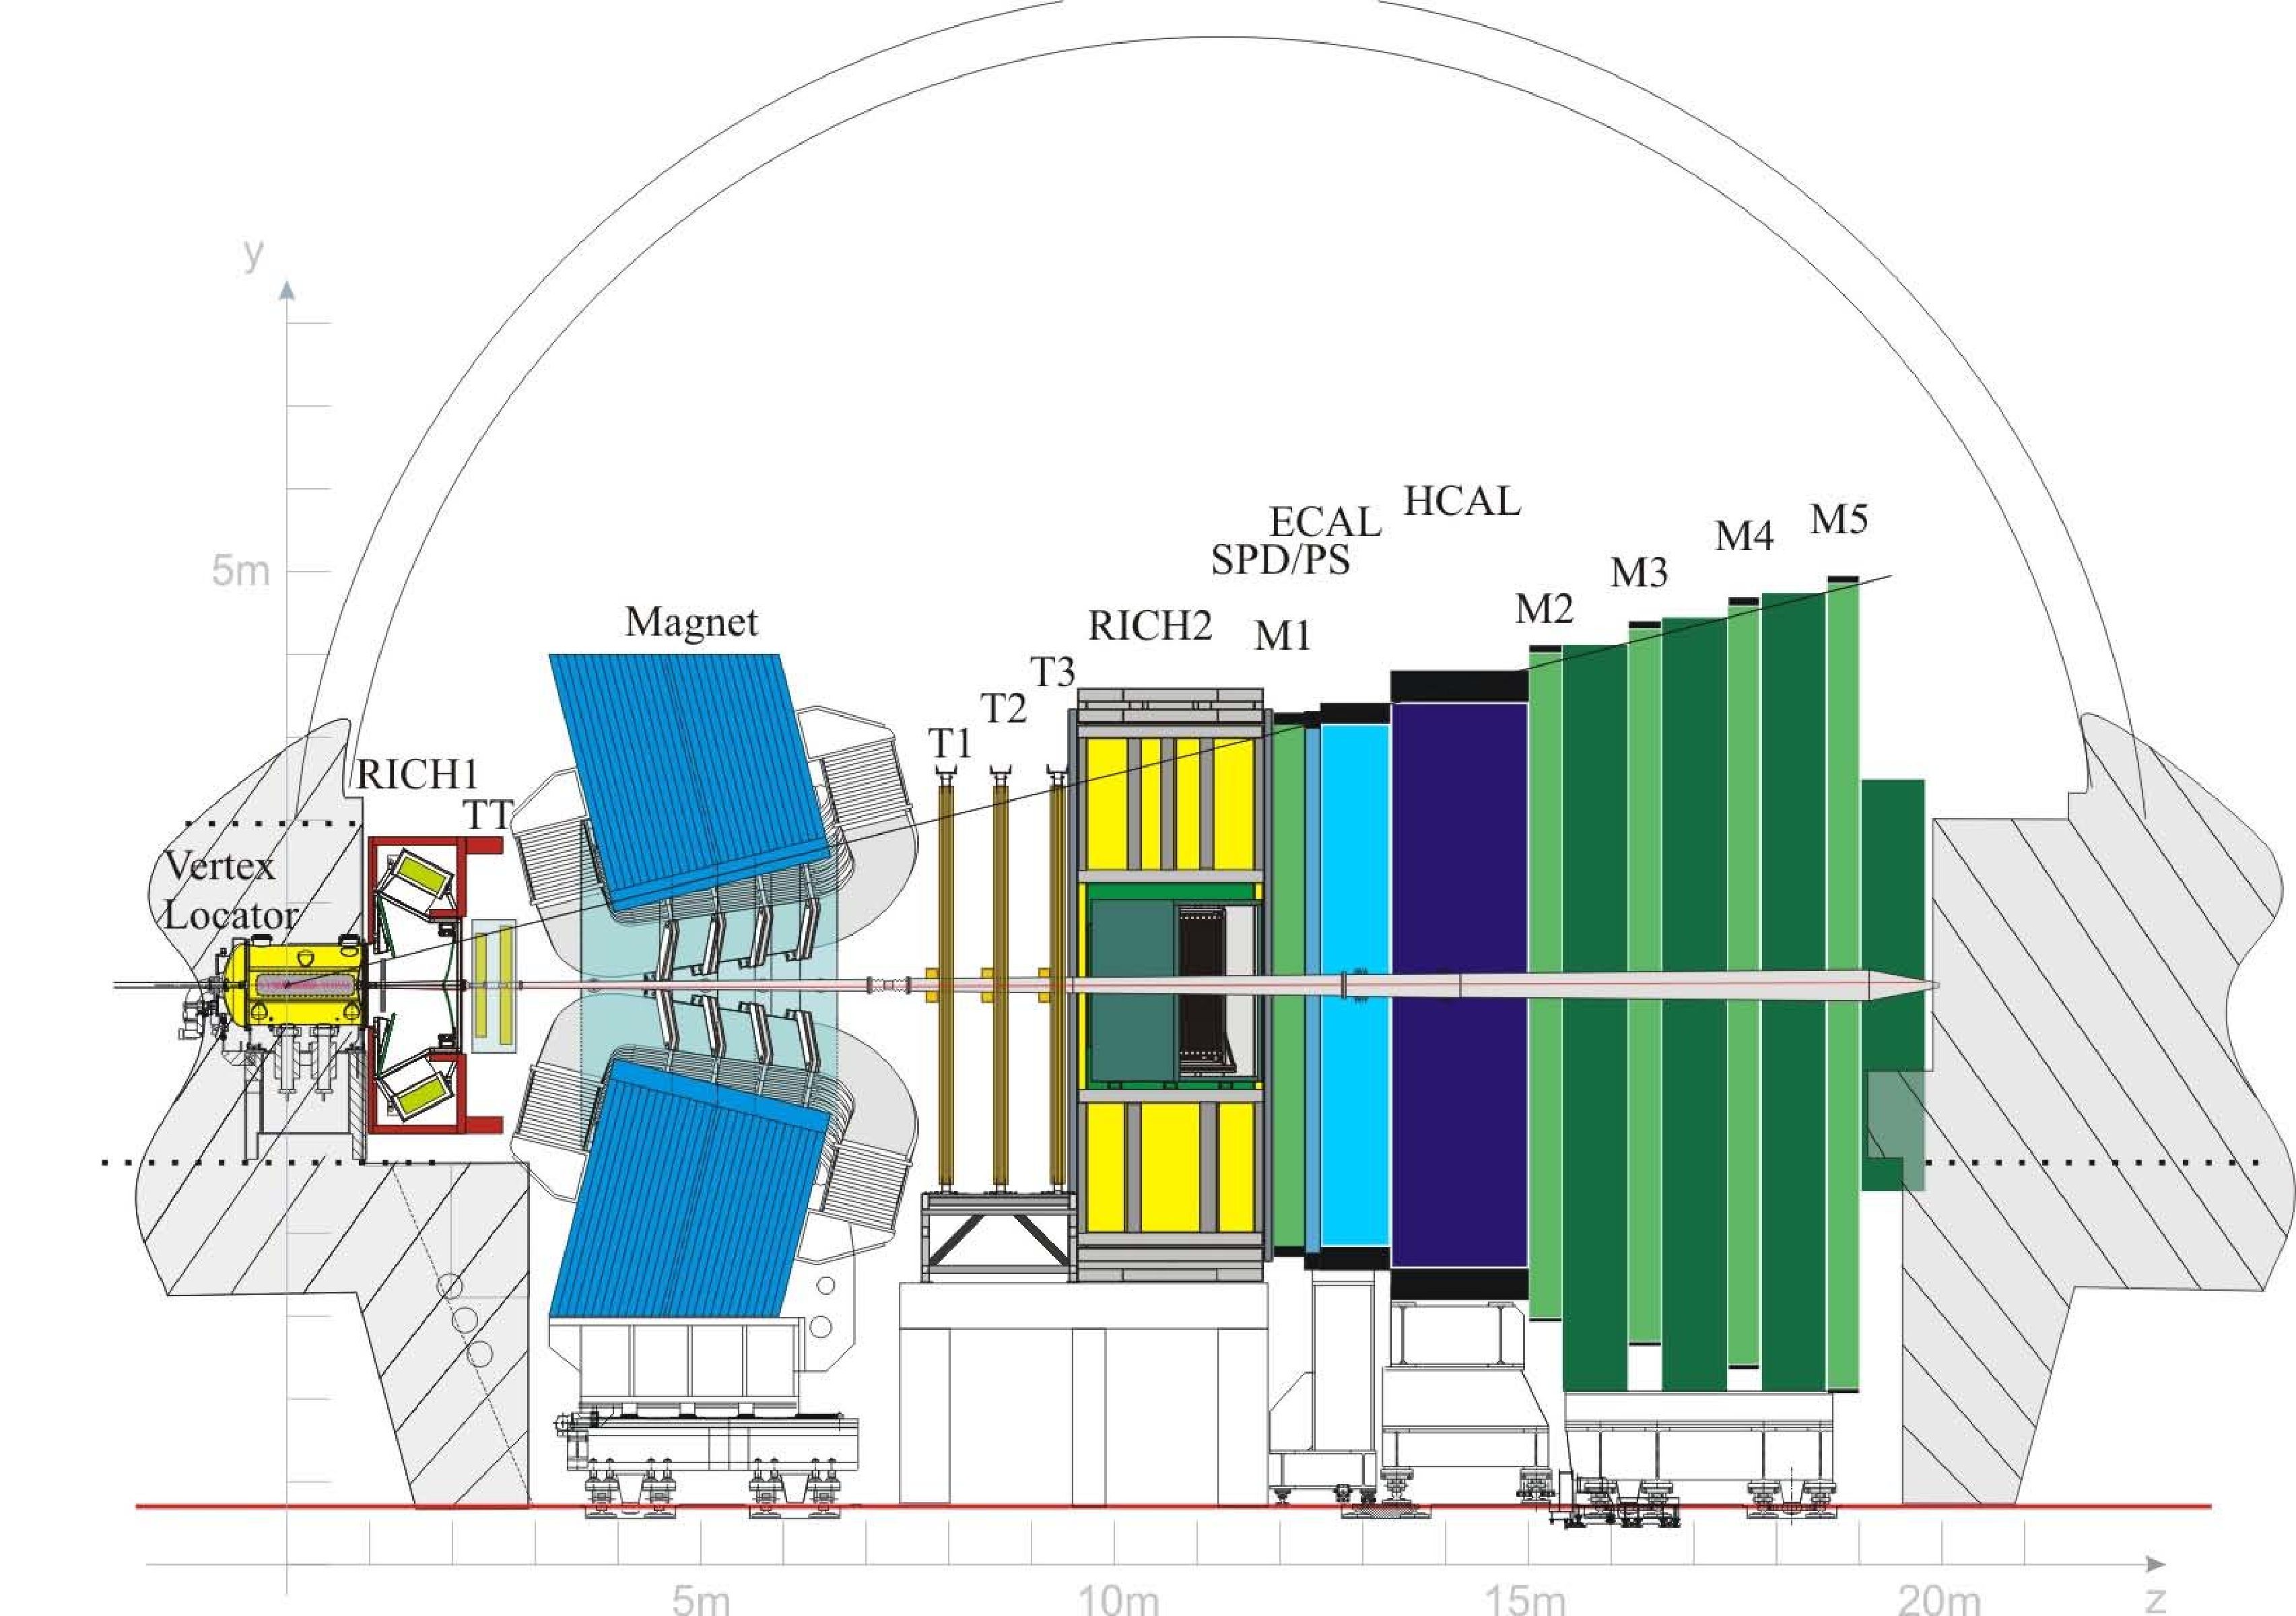
\includegraphics[scale = 0.15]{figs/detector/lhcbdet.pdf}
	\caption{The schematic slice of LHCb detector in $y,z$ plane where $z$ is defined to be the direction parallel to beamline, and $x,y$ define the plane perpendicular to the beamline. $\theta$, the opening angle in y-z plane with $\theta$ = 0 along $z-axis$. The figure was taken from \cite{LHCbdetector}.}
	\label{fig:LHCbDetector}
\end{figure}


To limit the background coming from especially soft QCD processes (due to hadronic collision enviroment) global event cuts, \textit{GEC}s, are put in the place. To limit the occupancy of the detector only events with 600 (in 7,8 \tev) and 450 (in 13 \tev) tracks and less are allowed to be processed. In order to achieve these occupancies, $\mu_{vis}$, the average number of visible $pp$ interactions per bunch-crossing is kept below 1, so that the pile-up, the visible number of $pp$ interaction in the visible events, is limited. This LHCb-specific control of luminosity is achieved by \textit{luminosity levelling}. This procedure achieves stable instantenous luminosity by controlling the transverse overlap of the beams at collision point. It limits the effects of luminosity decay, which can lead to trigger alterations during specific data taking run, resulting in systematic uncertainties.

So far, the detector has been running since 2010, with collected integrated luminosity shown in \autoref{fig:lhcbintlumi}. As compared to \Gls{ATLAS} and \Gls{CMS} the integrated luminosity is much lower, due to allowed pile-up conditions. In 2017, there were two $pp$ collision energies at which the data was taken: at $\sqrt(s)$  = 13 and 5 TeV. Run \Rn{1} data-taking (2010-2012) was paused by Long Shutdown 1 (\Gls{LS1}) and followed with Run \Rn{2} data-taking (2015-2018). 

%Formally LHCb detector is placed along the beamline, where $x,y,z$ a spectrometer which cover the region of 300 \mrad defined a
%http://lhcb.web.cern.ch/lhcb/speakersbureau/excel/default.html

%\begin{figure}
%	\centering
%	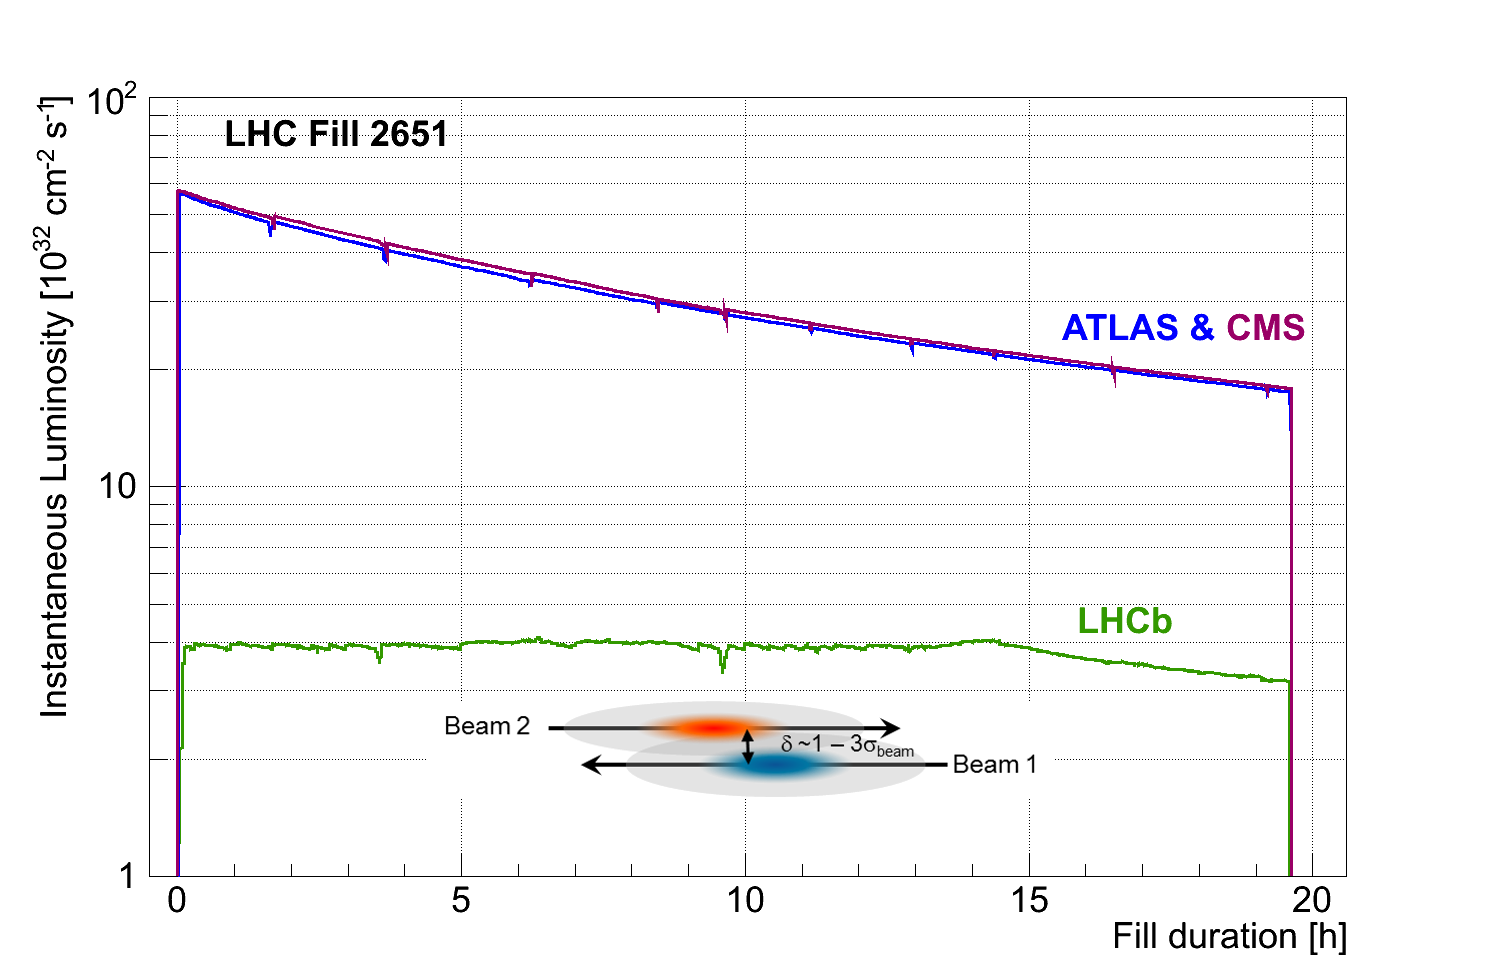
\includegraphics[scale = 0.5]{figs/detector/lumicompare.png}
%	\caption{Integrated luminosity collected in different years of data-taking. This plot is taken from \cite{lumiover}.}
%	\label{fig:lhcbintlumi}
%\end{figure}



%\begin{table}[!h]
%	\centering
%	\hspace*{-0.8cm}
%	\begin{tabular}{l c c c c }
%		\hline
%		 & $\sqrt(s)$ [TeV] & Luminosity $\mathcal{L}$ [$\times10^{32} cm^{-2}
%		s^{-1}$] & Number of Bunches & Bunch Spacing [ns] \\ \hline
%		2011 & 7  & 3.5 & 1300 &  50\\
%		2012 & 8 & 4 & 1300 &  50\\
%		2015 & 13 & 4 &  1.12 &  25\\      
%		2016 & 13 & 4 &  1.12 &  25\\      
%		2017 & 13 & 4 &  1.12 &  25\\\hline      
%	\end{tabular}
%	\caption{}
%	\label{tab:runcond}
%\end{table}   

\begin{figure}
	\centering
	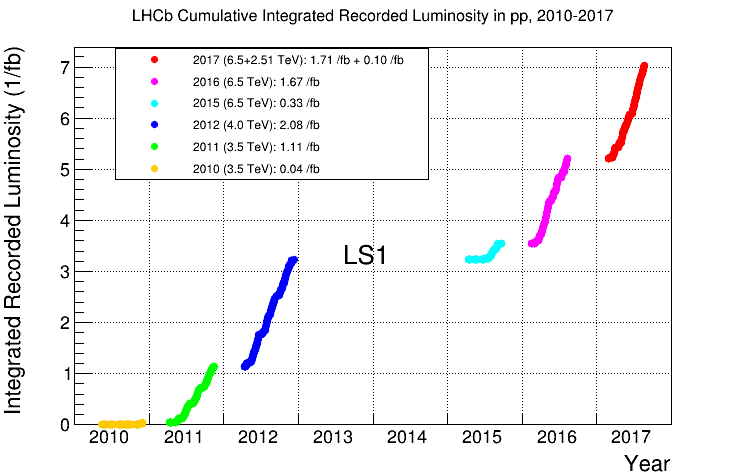
\includegraphics[width = 0.5\textwidth]{figs/detector/intlumi.png}%
        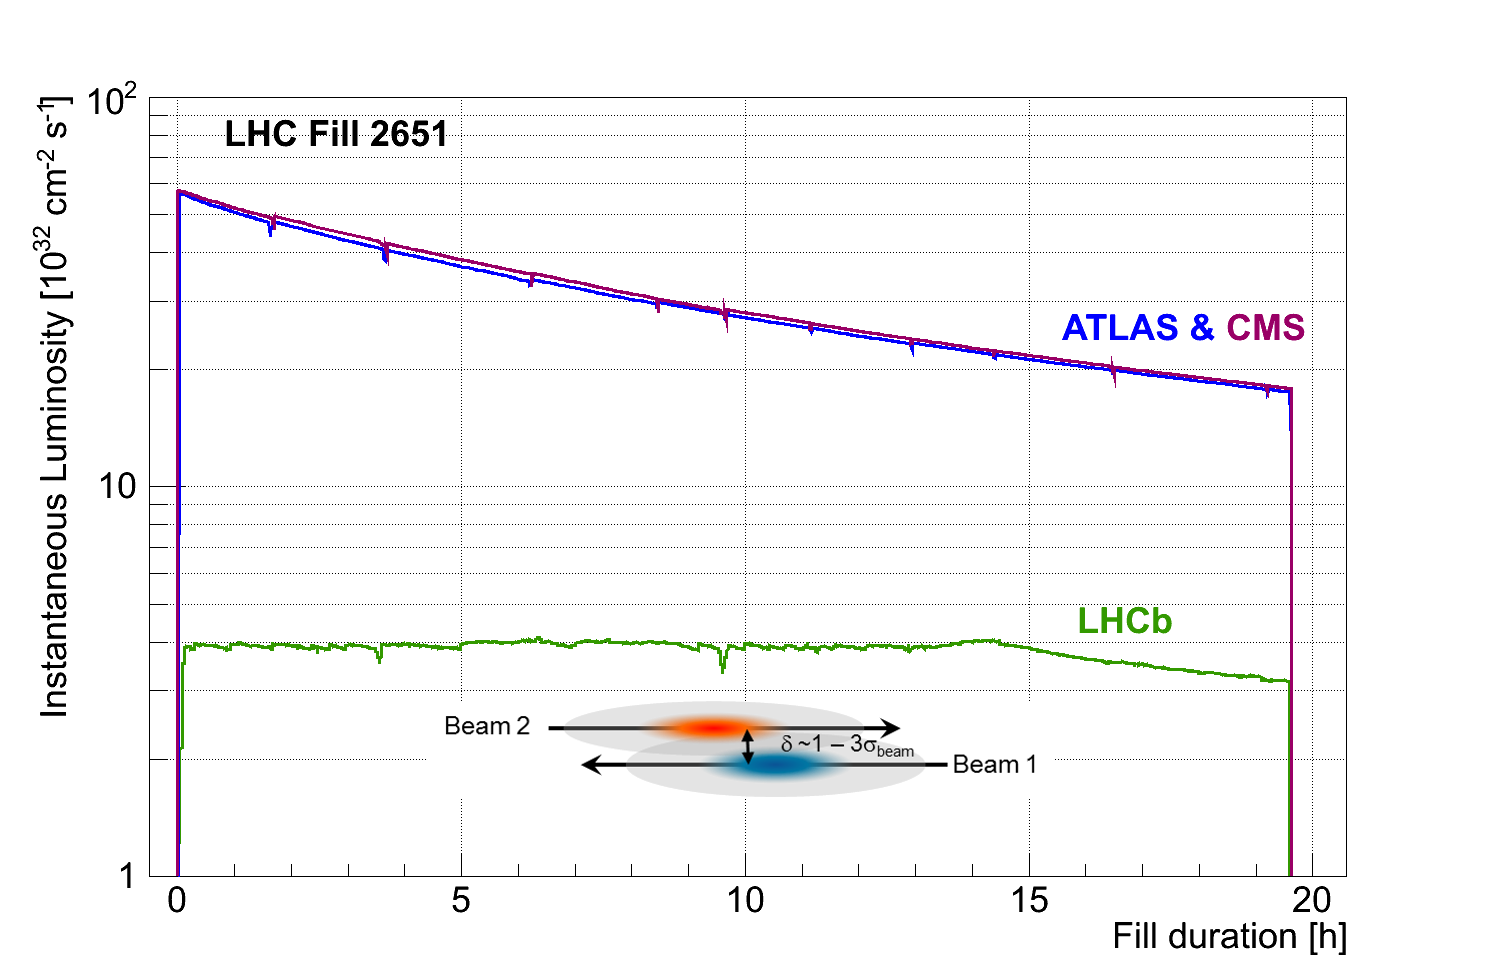
\includegraphics[width = 0.5\textwidth]{figs/detector/lumicompare.png}
	\caption{Integrated luminosity collected in different years of data-taking. This plot is taken from \cite{lumiover} (left). Development of the instantaneous luminosity for \Gls{ATLAS}, \Gls{CMS} and \Gls{LHCb} during LHC fill 2651. After ramping to the desired value of $4\times10^{32}cm^{-2}s^{-1}$
for LHCb, the luminosity is kept stable in a range of 5$\%$ for about 15 hours by adjusting the transversal beam overlap. The difference in luminosity towards the end of the fill between ATLAS, CMS and LHCb is due to the difference in the final focusing at the collision points, commonly referred to as the beta function, $\beta^{*}$. This plot was obtained from \cite{LHCb-DP-2014-002} (right).}
	\label{fig:lhcbintlumi}
\end{figure}

In the following sections, brief discussion of different subdetectors is presented. Both hardware and software overview will be presented with particular emphasis given to Muon Station and Simulation of LHCb.

\section{VErtex LOcator}
The closest detector around the collision point is VErtex LOcator (\Gls{VELO}). This silicon-strip based detector, that extends 1 \m along the beam axis, is primarily used for to distinguish events from promt background. The typical differing property of a $B$ hadron decay includes large impact parameter (\Gls{IP}), the minimal distance between the track and primary vertex, in addition to significantly higher transverse momentum $p_{T}$. 
\begin{itemize}
\item primary vertices positions
\item secondary vertices of short-lived particles (heavy quark hadrons)
\item tracks that did NOT originate from primary vertex
\end{itemize}.



 The detector consists of two sets of 21 silicon modules positioned around the beam pipe, where each module has 2 types of half-moon-shaped discs. In the first disc type the strips are arranged to provide radial information ($R$), whereas the second type provides azimuthal ($\phi$) information. As $pp$ interaction point brings high radiation dose for this detector, the first sensitive strip starts only at a distance of 8 \mm once stable beams are declared. Throughout the beam injection, when the beam radius may be larger, the two sets are moved away 3 \cm perpendicularly from the interaction point. For the ($R$) sensor The individual module's strip pitch, distance between two strips, varies from 38 $\mu m$ to 102 $\mu m$ away from the beam pipe, so that the hit occupancy is roughly even. This setup, which can be seen in \autoref{fig:veloover}, brings outstanding hit resolution (4-40$\mu m$). 

\begin{figure}[!h]
	\centering
	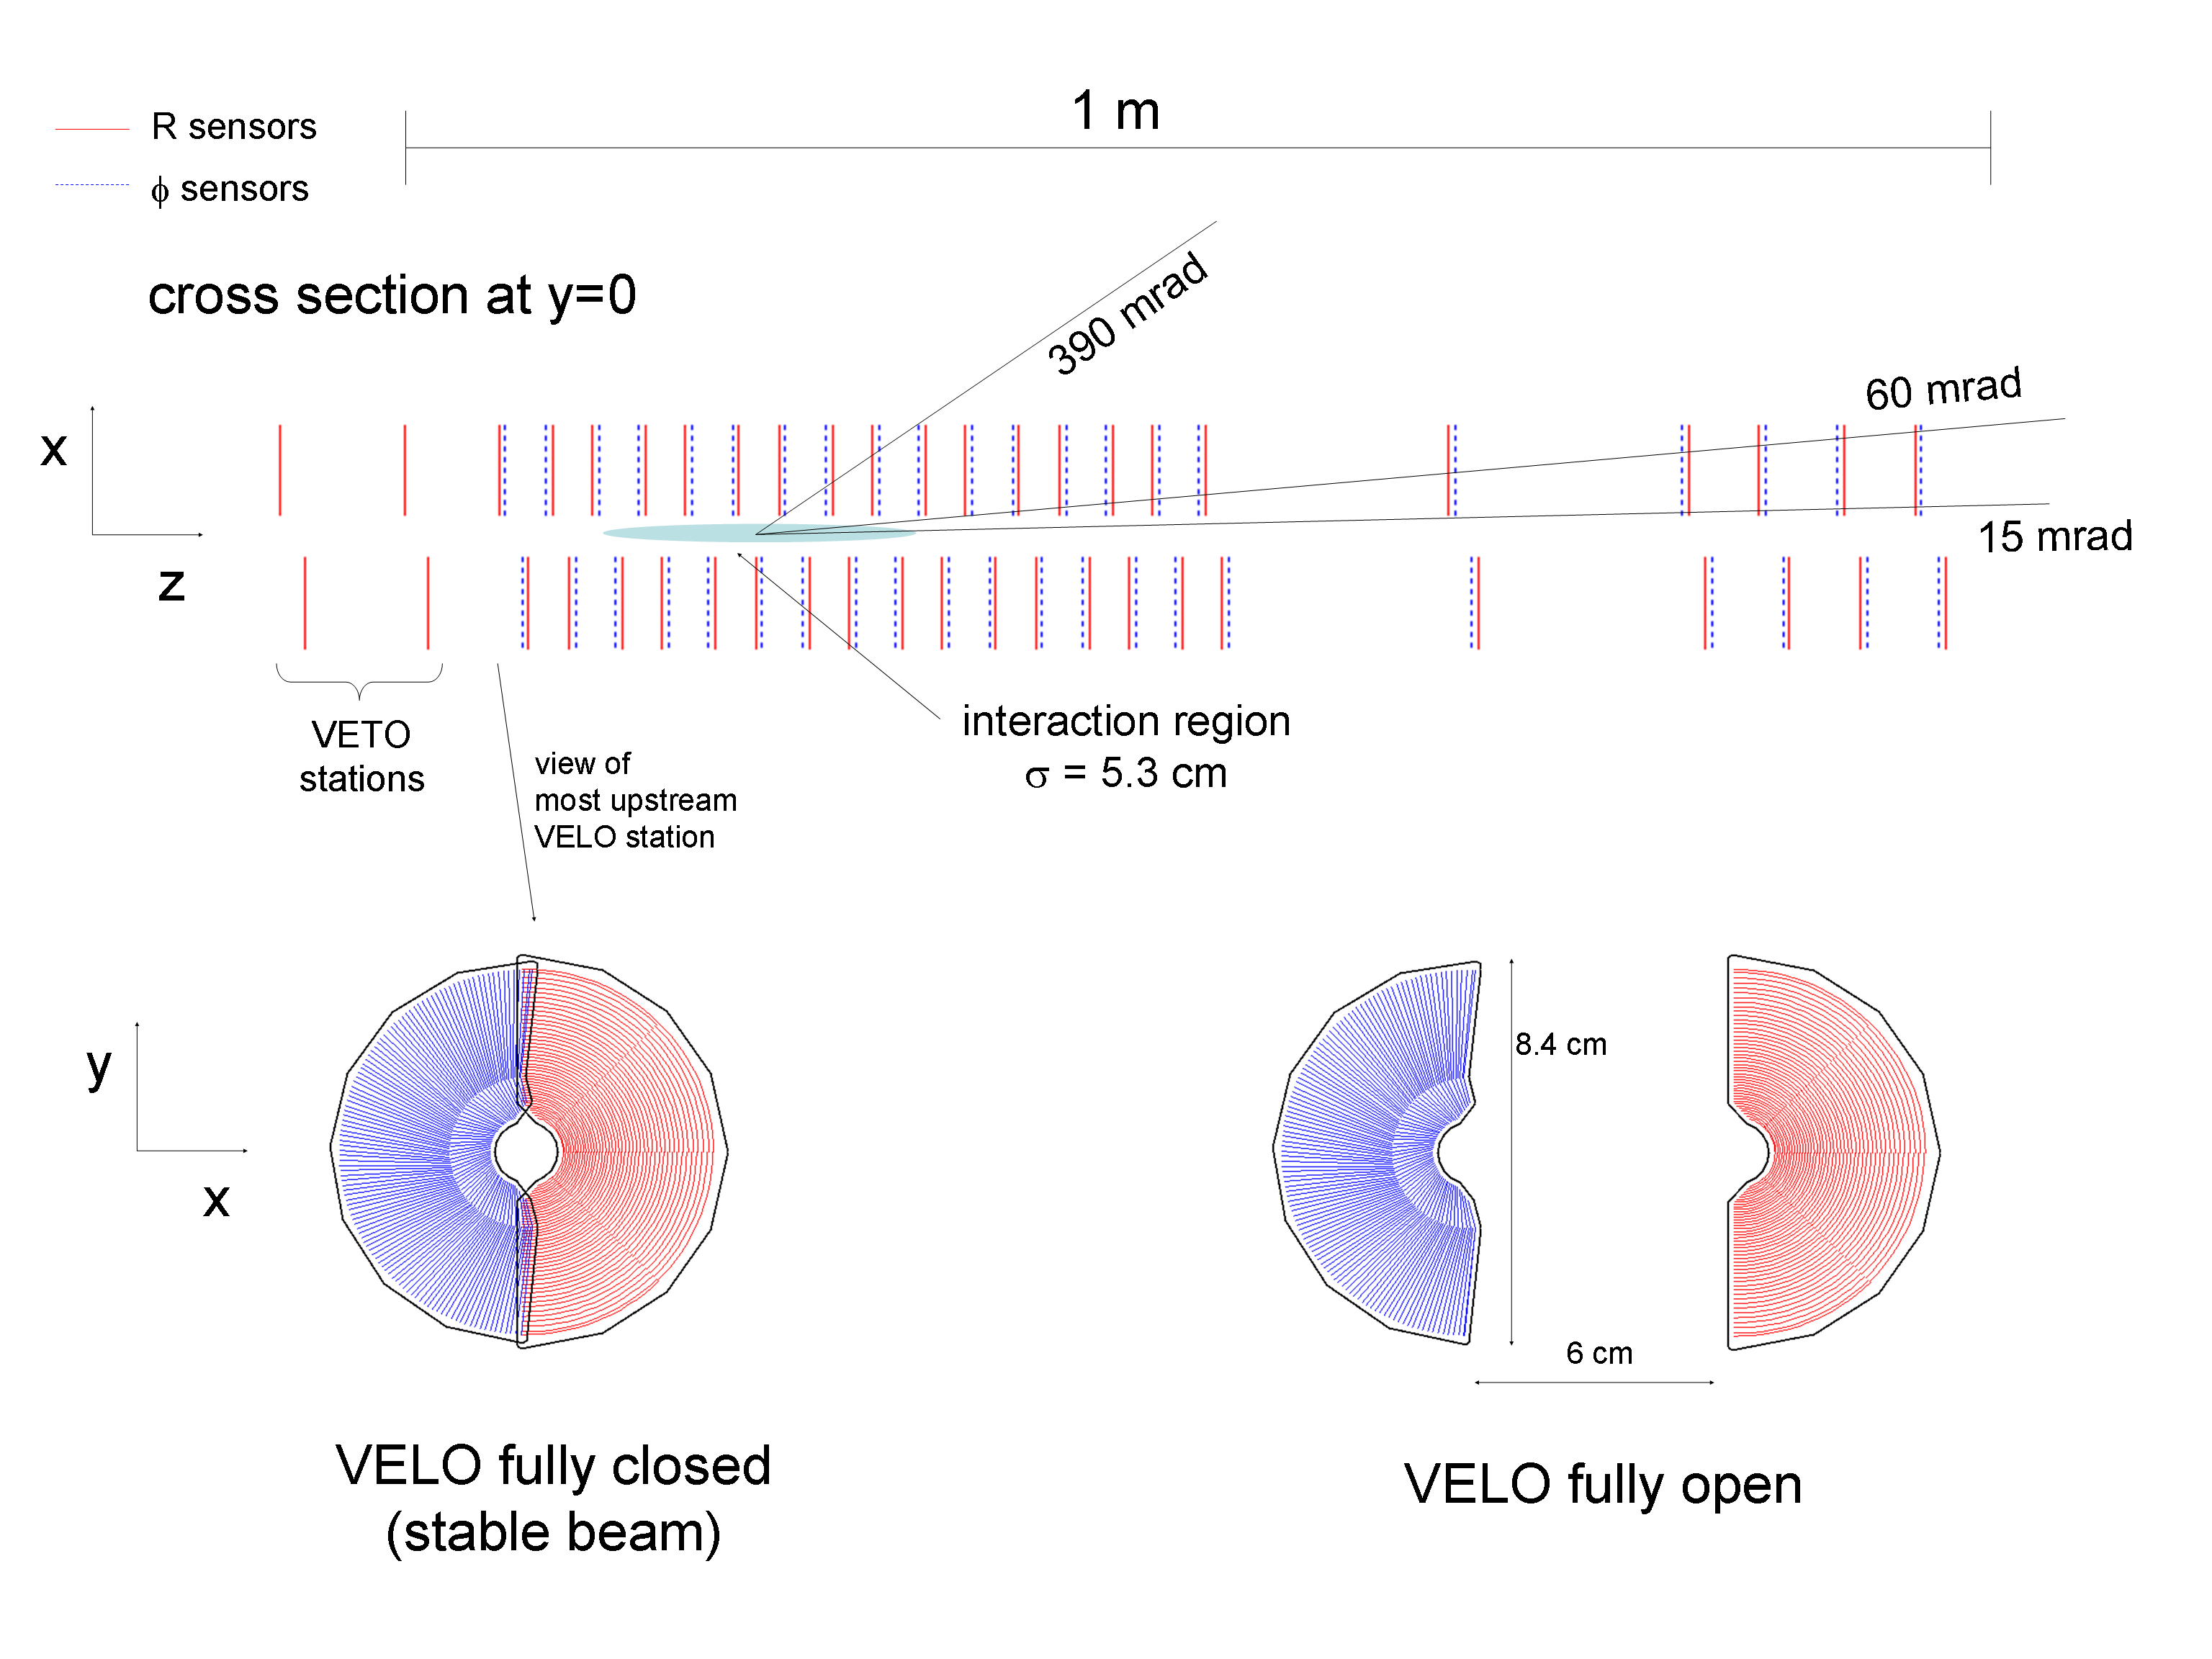
\includegraphics[width = 0.75\textwidth]{figs/detector/veloOverview.png}
        %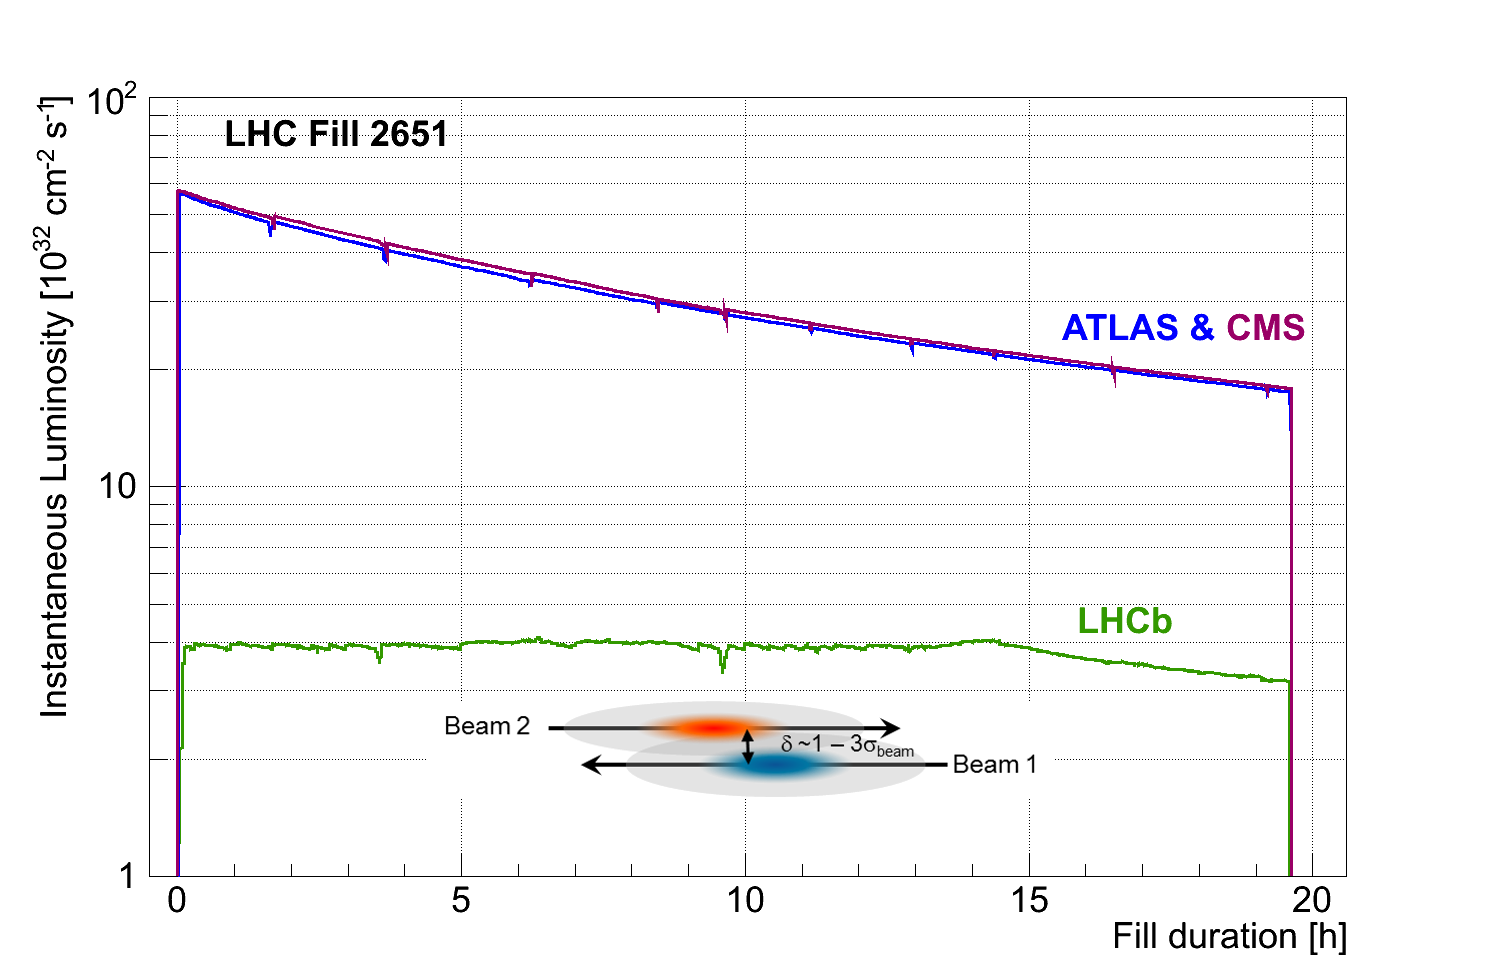
\includegraphics[width = 0.5\textwidth]{figs/detector/lumicompare.png}
	\caption{ Schematic plot of \Gls{VELO} detector configuration along the beam pipe showing the layout as well as positions while in stable beams (discs have slight overlap) and injection. Figure taken from \cite{det_paper}.}
	\label{fig:veloover}
\end{figure}


\section{Tracking System}
In addition to tracking information provided by \Gls{VELO}, the trajectories of charged particles are monitored by series of tracking subdetectors. The main task of these tracking subdetectors is to provide efficient reconstruction and precise measurement of particle's momentum. There are four tracking stations apart from \Gls{VELO}: Tracker Turicensis (\Gls{TT}), positioned upstream from magnet, and  \Gls{Tstation} tracking stations on the other side from the magnet. The 10 \m dipole magnet with $\approx$ 4 Tm integrated field provides enough strenght to bend charged particles with $p$ of 200 $GeV/c^{2}$.      

 Two different dectection technologies are used in these trackers reflecting the nature of track occupancy as function of distance from beam pipe. The tracker's part close to the beam pipe, \Gls{TT} station together with central region of T1-T3 (Inner Tracker (\Gls{IT}) expects higher occupancy, making use of the the silicon microstrip detection mechanism. The outer part of \Gls{Tstation} stations, also known as outer tracker \Gls{OT}, is made of a straw-tube detectors. It measures the hit position by measuring the drift-time of ionized electrons. This two technologies are seen in  

\subsection{Tracking Algorithms}
   Altogether, there are several track categories, that can be formed visualized in \autoref{fig:tracktype}. 


\begin{figure}[!h]
	\centering
	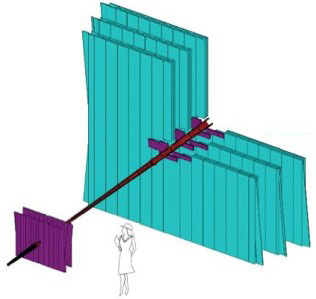
\includegraphics[width = 0.35\textwidth]{figs/detector/trackingsystem.jpg}%
	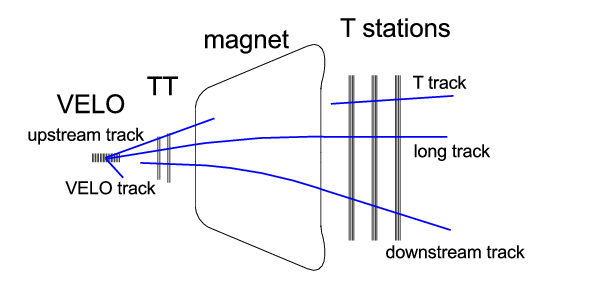
\includegraphics[width = 0.6\textwidth]{figs/detector/tracktype.png}
	\caption{ Visualisation of use of different technology with silicon technology in violet and straw-tube technology in cyan \cite{OT}. The Figure was obtained in  (left). Track types visualisation depending on which track stations provided hits. Figure is taken from \cite{LHCb-DP-2013-002}. For the study of \Bmumumu decay only long tracks are considered (right). }
	\label{fig:tracktype}
\end{figure}


